% % \begin{tikzpicture}[
%     % Global settings for a more compact layout
%     node distance=2mm and 5mm,
%     % --- STYLES ---
%     outerbox/.style={
%         draw, 
%         rectangle, 
%         minimum width=9cm, 
%         minimum height=10.5cm, 
%         line width=0.5pt
%     },
%     innerbox/.style={
%         draw, 
%         rectangle, 
%         minimum width=8cm, 
%         line width=0.5pt, 
%         fill=gray!5
%     },
%     boxtitle/.style={
%         font=\small\bfseries, 
%         text centered
%     },
%     boxsubtitle/.style={
%         font=\small\itshape, 
%         text centered, 
%         text width=6.5cm
%     },
%     listtext/.style={
%         font=\small, 
%         align=left
%     },
%     boundarytext/.style={
%         font=\small, 
%         fill=white, % White fill to sit cleanly over the line
%         inner sep=2pt
%     },
%     sidelabel/.style={
%         font=\small\itshape, 
%         align=left
%     },
%     boundaryline/.style={
%         draw, 
%         double, 
%         thick, 
%         gray!80
%     },
%     vertical_arrow/.style={
%         <->, % Bidirectional arrow
%         thick,
%         >=latex % Arrowhead style
%     }
% ]

% % 1. Main outer box and its title
% \node[outerbox] (main) {};
% \node[boxtitle, anchor=north, yshift=-4mm] at (main.north) {System Environment};
% \node[boxsubtitle, below=1mm of main.north] at (main.north) {(Operating System, Containers, Services)};

% % 2. Top inner box (Agent Runtime)
% \node[innerbox, minimum height=3cm, anchor=north, yshift=-1.8cm] (agent) at (main.north) {};
% \node[boxtitle, anchor=north, yshift=-4mm] at (agent.north) {Agent Runtime Framework};
% \node[boxsubtitle, anchor=north, yshift=-9mm] at (agent.north) {(LangChain, AutoGen, Claude Code)};
% \node[listtext, anchor=center, yshift=-4mm] at (agent.center) {
%     \textbullet~Prompt orchestration \\
%     \textbullet~Tool execution logic \\
%     \textbullet~State management
% };

% % 3. Bottom inner box (LLM Service)
% \node[innerbox, minimum height=1.6cm, anchor=south, yshift=2.8cm] (llm) at (main.south) {};
% \node[boxtitle, anchor=north, yshift=-4mm] at (llm.north) {LLM Service Provider};
% \node[boxsubtitle, anchor=north, yshift=-9mm] at (llm.north) {(OpenAI API, Local Models)};

% % 4. Define boundary line positions
% \coordinate (net_boundary_pos) at ($(agent.south)!0.5!(llm.north)$);
% \coordinate (kern_boundary_pos) at ($(llm.south) + (0, -1.2cm)$);

% % 5. Draw Network Boundary and its elements
% \draw[boundaryline] (main.west |- net_boundary_pos) -- (main.east |- net_boundary_pos);
% \node[boundarytext, below=1mm of net_boundary_pos] (net_text) {(TLS-encrypted traffic)};
% \draw[vertical_arrow] ($(agent.south)+(0,-2mm)$) -- ($(net_boundary_pos)+(0,2mm)$);
% \draw[vertical_arrow] ($(llm.north)+(0,2mm)$) -- ($(net_boundary_pos)-(0,2mm)$);

% % 6. Draw Kernel Boundary and its text
% \draw[boundaryline] (main.west |- kern_boundary_pos) -- (main.east |- kern_boundary_pos);
% \node[boundarytext, below=1mm of kern_boundary_pos] (kern_text) {(System calls, File I/O)};

% % 7. Add side labels with arrows pointing to the elements
% \node[sidelabel, anchor=west] (app_label) at ($(agent.east) + (0.8cm, 0.2cm)$) {Application Layer};
% \draw[<-] (app_label.west) -- ($(app_label.west) - (0.6, 0)$);

% \node[sidelabel, anchor=west] (net_label) at ($(main.east |- net_boundary_pos) + (0.8cm, 0.2cm)$) {Network Boundary};
% \node[sidelabel, anchor=north west] at (net_label.south west) {(Observable)};
% \draw[<-] (net_label.west) -- ($(net_label.west) - (0.6, 0)$);

% \node[sidelabel, anchor=west] (kern_label) at ($(main.east |- kern_boundary_pos) + (0.8cm, 0.2cm)$) {Kernel Boundary};
% \node[sidelabel, anchor=north west] at (kern_label.south west) {(Observable)};
% \draw[<-] (kern_label.west) -- ($(kern_label.west) - (0.6, 0)$);

% \end{tikzpicture}


% \begin{center}
% \begin{Verbatim}[fontsize=\small, commandchars=\\\{\}]
% ┌─────────────────────────────────────────────────┐
% │             System Environment                  │
% │  (Operating System, Containers, Services)       │
% │                                                 │
% │  ┌─────────────────────────────────────────┐   │
% │  │      Agent Runtime Framework            │   │  ← Application Layer
% │  │   (LangChain, AutoGen, Claude Code)     │   │
% │  │   • Prompt, tool, memory                │   │
% │  └─────────────────────────────────────────┘   │
% │                    ↕                            │
% │  ═══════════════════════════════════════════   │  ← Network Boundary
% │           (TLS-encrypted traffic)               │     (Observable)
% │                    ↕                            │
% │  ┌─────────────────────────────────────────┐   │
% │  │         LLM Service Provider            │   │
% │  │    (OpenAI API, Local Models)           │   │
% │  └─────────────────────────────────────────┘   │
% │                                                 │
% │  ═══════════════════════════════════════════   │  ← Kernel Boundary
% │         (System calls, File I/O, process)       │     (Observable)
% └─────────────────────────────────────────────────┘
% \end{Verbatim}
% \end{center}

\section{Design}

The design of AgentSight is guided by a single imperative: to bridge the semantic gap between an agent's intent and its actions. We achieve this through a novel observability method, boundary tracing, realized by a multi-signal correlation engine.

\subsection{Challenges}

The emergent and non-deterministic nature of AI agents fundamentally breaks traditional program observability paradigms, introducing two core challenges that original observability cannot address.

\textbf{Bridging the Semantic Gap Between Intent and Action}
The first and most significant challenge is bridging the vast semantic gap between an agent's high-level \textit{intent} and its low-level system \textit{actions}. Unlike conventional software, where intent is encoded in predictable source code, an agent's intent is expressed in natural language and interpreted by an LLM, creating dynamic "source code" that is generated at runtime. Consequently, it is impossible for a static analyzer to determine what an agent will do. For example, the intent "find and fix the bug in the authentication module" is semantically rich but operationally ambiguous, potentially resulting in a complex sequence of actions like reading files (\texttt{openat2}), compiling code (\texttt{execve} -> \texttt{gcc}), and running tests (\texttt{execve} -> \texttt{python}). This creates a critical observability problem: how can a monitoring system verify that the cascade of system calls is a legitimate fulfillment of the natural language intent? To solve this, an observer must move beyond simple pattern matching to gain a semantic understanding of the agent's goal, necessitating a new, llm based approach to interpret the correlated traces.

\textbf{Isolating the Causal Signal from High-Volume System Noise}
The second challenge stems from the agent's autonomy to use any tool necessary to achieve its goal, leading to an unpredictable and high-volume stream of system events. An agent might spawn shells, download scripts, or invoke compilers-processes that are not known ahead of time. This makes it exceedingly difficult to distinguish the agent's specific activity (the "signal") from the background noise of the operating system. Static, pre-configured filters, for instance, a rule to only monitor \texttt{git} commands, are inherently brittle and will fail the moment the agent uses \texttt{curl} and \texttt{bash} to achieve a similar outcome. Our design addresses this with an aggressive, dynamic in-kernel eBPF filter. By tracking process creation events (\texttt{fork}, \texttt{execve}), the filter builds a complete lineage tree of the agent's activity and dynamically applies rules in the kernel to only pass events from the agent or its descendants to userspace. This approach ensures that the entire causal chain is captured efficiently at the source, dramatically reducing overhead and providing a clean, high-fidelity signal for correlation and analysis.

\subsection{Boundary Tracing: A Principled Approach}

Our key insight is that all agent interactions must traverse well-defined and stable system boundaries: the kernel for system operations and the network for external communications with LLM serving backends (Figure \ref{fig:agent}). By monitoring at these boundaries rather than within volatile agent code, we achieve comprehensive monitoring independent of implementation details. This approach enables Semantic Correlation, the ability to causally link high-level intentions with low-level system events. This is supported by two principles. First is Comprehensiveness, as kernel-level monitoring ensures no system action from process creation to file I/O goes unobserved, even across spawned subprocesses. Second is Stability, since system call ABIs and network protocols evolve far more slowly than agent frameworks, providing a durable, future-proof solution. This paradigm shifts the trust model from assuming a cooperative agent to enforcing observation at tamper-proof boundaries.

\begin{figure}[h!]
    \centering
    % It is highly recommended to create this diagram using a tool like TikZ, Inkscape, or another vector graphics editor for the final paper.
    % The following is a LaTeX description of the recommended figure.
    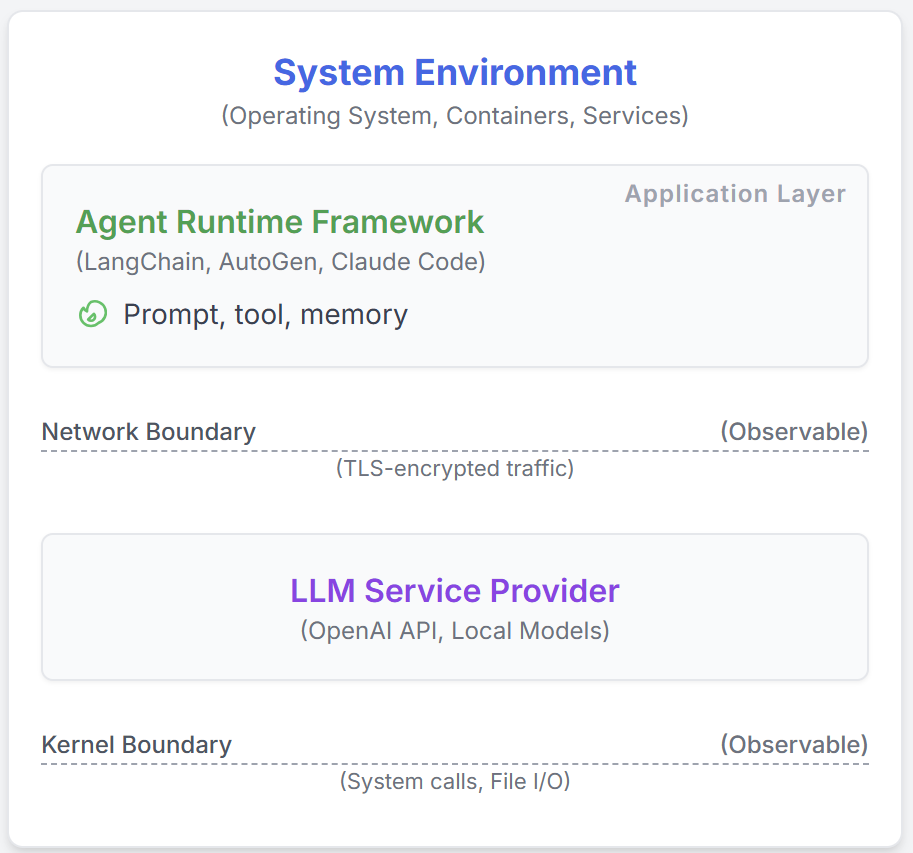
\includegraphics[width=\columnwidth]{figture/agent.png}
    \caption{Agent Framework Overview}
    \label{fig:agent}
\end{figure}

\subsection{System Architecture: Observing the Boundaries}

AgentSight's architecture simultaneously taps into the two critical boundaries. As shown in Figure \ref{fig:architecture}, we use eBPF to place non-intrusive probes that capture a decrypted Intent Stream (LLM prompts/responses) from userspace SSL functions and an Action Stream (syscalls, process events) from the kernel. A userspace correlation engine then processes and joins these streams into a unified, causally-linked trace.

\begin{figure}[h!]
    \centering
    % It is highly recommended to create this diagram using a tool like TikZ, Inkscape, or another vector graphics editor for the final paper.
    % The following is a LaTeX description of the recommended figure.
    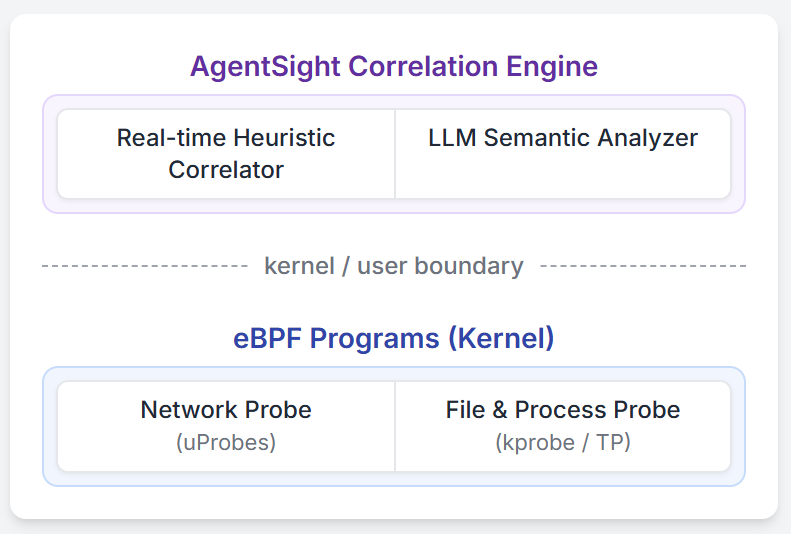
\includegraphics[width=\columnwidth]{figture/arch.png} % Replace with your actual figure file
    \caption{\textbf{AgentSight System Architecture.}}
    \label{fig:architecture}
\end{figure}

Several key components enable AgentSight to effectively bridge the semantic gap:

\textbf{eBPF for Safe, Unified Probing:} We chose eBPF for its production safety, high performance, and unified ability to access both userspace and kernel data streams. Our design intercepts decrypted data from the agent's interaction with LLM serving backend, which is more efficient and manageable than network-level packet capture or proxy-based solutions.

\textbf{Multi-Signal Causal Correlation Engine:} The core of our design is a correlation strategy that establishes causality between intent and action. We designed a multi-signal engine that relies on three key mechanisms: Process Lineage, which builds a complete process tree by tracking \texttt{fork} and \texttt{execve} events to link actions in child processes back to the parent agent; Temporal Proximity, which associates actions that occur within a narrow time window immediately following an LLM response; and Argument Matching, which directly matches content from LLM responses, such as filenames, URLs, or commands, with the arguments of subsequent system calls. Together, these signals enable AgentSight to definitively establish causal relationships between high-level intentions and low-level system operations across process boundaries.

\textbf{LLM-Powered Semantic Analysis:} To move beyond brittle, rule-based detection, we designed the system to use a secondary LLM as a reasoning engine. By prompting a powerful model with the correlated event trace, we leverage its ability to understand semantic nuance, infer causality in complex scenarios, and summarize findings in natural language. This "AI to watch AI" approach allows AgentSight to detect threats that do not match predefined patterns.

\section{Implementation}

AgentSight is implemented as a userspace daemon (6000 lines of Rust/C) orchestrating eBPF programs, with a TypeScript frontend (3000 lines) for analysis. It is designed for high performance, processing raw kernel event streams into correlated, human-readable data.

\subsection{Data Collection at the Boundaries}

Our eBPF probes capture the raw intent and action streams from the system. To capture semantic intent, an eBPF program with uprobes attaches to SSL\_read/SSL\_write in crypto libraries like OpenSSL to intercept decrypted LLM communications. Our userspace daemon implements a stateful reassembly mechanism to handle streaming protocols such as Server-Sent Events (SSE). To capture system actions, a second eBPF program uses stable tracepoints like sched\_process\_exec to build a process tree and kprobes to dynamically monitor relevant syscalls such as openat2, connect, and execve. To manage the high volume of kernel events without data loss, aggressive in-kernel filtering is applied to ensure only events from targeted agent processes are sent to userspace, minimizing overhead.

\subsection{The Hybrid Correlation Engine}

The Rust-based userspace daemon houses our two-stage correlation engine. The first stage consumes events from eBPF ring buffers and performs real-time heuristic linking. This streaming pipeline enriches raw events with context like mapping a file descriptor to a full path, maintains a stateful process tree, and applies the causal linking logic described in our design, using a 100-500ms window for temporal correlation. Once a coherent trace is constructed, the second stage formats it into a structured log for semantic analysis. This log is used to construct a detailed prompt for a secondary LLM, instructing it to act as a security analyst. The LLM's natural language analysis and confidence score become the final output of our system. A key challenge at this stage is managing the latency and cost of LLM analysis, which our system mitigates through asynchronous processing and robust prompt engineering.

% \section{Design}

% The design of AgentSight is guided by a single imperative: to bridge the semantic gap between an agent's intent and its actions. We achieve this through a novel observability method, \emph{boundary tracing}, which is built on a foundation of stable system interfaces and realized through a multi-signal correlation engine.

% \subsection{Boundary Tracing: A Principled Approach}

% We propose \emph{boundary tracing} as a novel approach to AI agent observability. The key insight is that all meaningful agent interactions must traverse well-defined system boundaries: the kernel interface for system operations and the network interface for external communications, as shown in figture \ref{fig:agent}. By observing at these boundaries rather than within agent code, we achieve stable, comprehensive monitoring independent of agent implementation details.

% The primary goal of this approach is to enable {Semantic Correlation}, the ability to causally link high-level intentions with low-level system events. This goal is made possible by two foundational principles: {Comprehensiveness}, where by monitoring at the kernel we ensure that no system-level action, including process creation and file I/O, can go unobserved, regardless of the agent's implementation language or its attempts to evade monitoring by spawning subprocesses; and {Stability}, where system call ABIs and network protocols evolve far more slowly than agent frameworks, providing a durable solution resilient to the constant breaking changes common in agent libraries. This paradigm fundamentally shifts the trust model from assuming a cooperative agent to enforcing observation at tamper-proof system boundaries.

% \begin{figure}[h!]
%     \centering
%     % It is highly recommended to create this diagram using a tool like TikZ, Inkscape, or another vector graphics editor for the final paper.
%     % The following is a LaTeX description of the recommended figure.
%     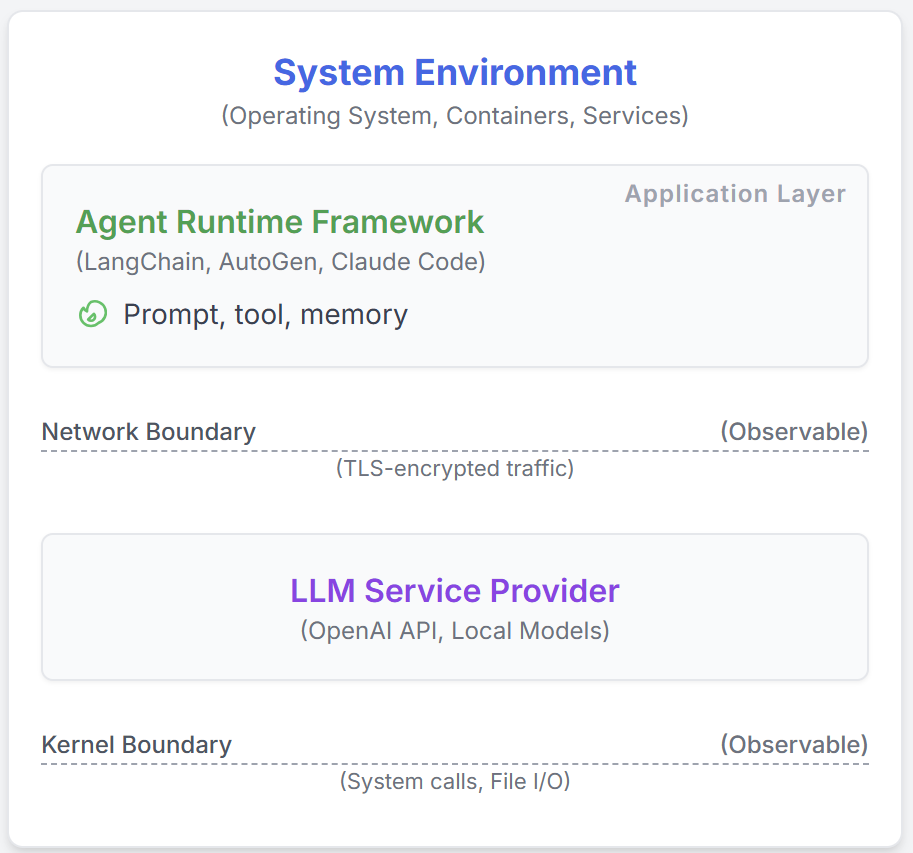
\includegraphics[width=\columnwidth]{figture/agent.png}
%     \caption{agent framwork overview}
%     \label{fig:agent}
% \end{figure}

% \subsection{System Architecture: Observing the Boundaries}
% AgentSight's architecture is designed to simultaneously tap into the two critical boundaries an agent interacts with: the network boundary for semantic intent and the kernel boundary for system actions. Figure \ref{fig:architecture} illustrates this architecture. We use eBPF to place non-intrusive probes at both boundaries. Probes on SSL library functions in userspace capture the decrypted **Intent Stream** (LLM prompts and responses), while probes at the kernel level capture the **Action Stream** (syscalls, process events). Both streams are processed by our userspace correlation engine, which joins them to produce a unified, causally-linked event trace.

% \begin{figure}[h!]
%     \centering
%     % It is highly recommended to create this diagram using a tool like TikZ, Inkscape, or another vector graphics editor for the final paper.
%     % The following is a LaTeX description of the recommended figure.
%     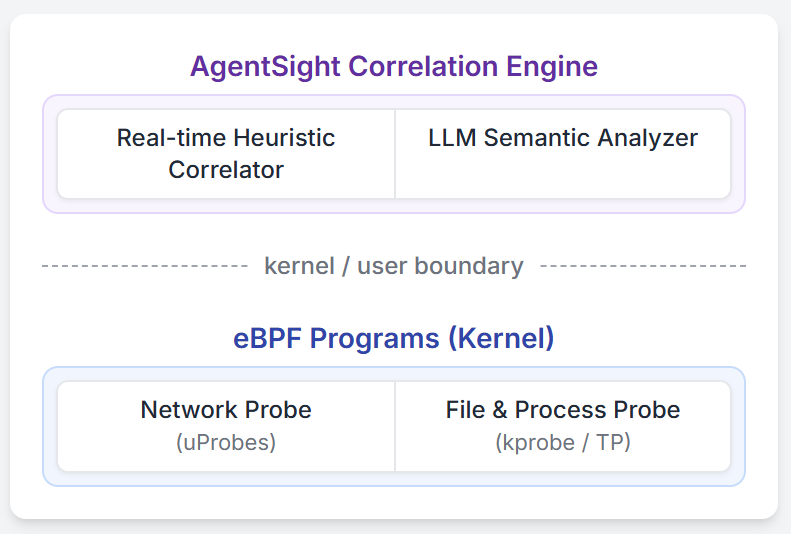
\includegraphics[width=\columnwidth]{figture/arch.png} % Replace with your actual figure file
%     \caption{\textbf{AgentSight System Architecture.}}
%     \label{fig:architecture}
% \end{figure}

% \subsection{Core Components}

% Several key decisions enable AgentSight to effectively bridge the semantic gap:

% \textbf{eBPF for Safe, Unified Probing:} We chose eBPF because it provides a single, production-safe technology to access both userspace and kernel data streams. Its verified safety model eliminates the risks of kernel modules, and its performance is vastly superior to traditional userspace hooking or \texttt{ptrace}-based approaches. For semantic intent, our design specifies intercepting decrypted data directly from the agent's memory. This is superior to network-level packet capture, as it avoids TLS key management, and more efficient than proxy-based solutions.

% \textbf{Multi-Signal Causal Correlation Engine:} The core of our design is a correlation strategy that establishes causality between intent and action. We designed a multi-signal engine that relies on three key mechanisms: Process Lineage, which builds a complete process tree by tracking \texttt{fork} and \texttt{execve} events to link actions in child processes back to the parent agent; Temporal Proximity, which associates actions that occur within a narrow time window immediately following an LLM response; and Argument Matching, which directly matches content from LLM responses, such as filenames, URLs, or commands, with the arguments of subsequent system calls. Together, these signals enable AgentSight to definitively establish causal relationships between high-level intentions and low-level system operations across process boundaries.

% \textbf{LLM-Powered Semantic Analysis:} To move beyond brittle, rule-based detection, we designed the system to use a secondary LLM as a reasoning engine. By prompting a powerful model with the correlated event trace, we leverage its ability to understand semantic nuance, infer causality in complex scenarios, and summarize findings in natural language. This "AI to watch AI" approach allows AgentSight to detect threats that do not match predefined patterns.

% \section{Implementation}

% AgentSight is implemented as a userspace daemon written in 6000 line Rust and C that orchestrates a suite of eBPF programs, with a 3000 line typescript frontend for visualization and analysis. The system is designed for high performance and low overhead, processing raw event streams from the kernel to produce correlated, human-readable observability data.

% \subsection{Data Collection at the Boundaries}
% Our eBPF probes are responsible for capturing the raw intent and action streams from the system.

% \textbf{Capturing Semantic Intent (TLS):} An eBPF program utilizing \texttt{uprobes} is attached to \texttt{SSL\_read} and \texttt{SSL\_write} functions in dynamically linked crypto libraries (e.g., OpenSSL, BoringSSL). This allows us to intercept all decrypted LLM communications. A significant challenge here is handling streaming protocols like Server-Sent Events (SSE), which fragment a single JSON response across numerous \texttt{SSL\_read} calls. Our userspace daemon implements a stateful reassembly mechanism that buffers data chunks per-connection and parses them for event boundaries (double newlines) to reconstruct complete messages.

% \textbf{Capturing System Actions (Kernel):} A second eBPF program monitors kernel activity. We use efficient, stable \texttt{tracepoints} like \texttt{sched\_process\_fork} and \texttt{sched\_process\_exit} to build a process tree. For detailed actions, we use \texttt{kprobes} to dynamically attach to specific system calls relevant to agent behavior, such as \texttt{openat2} (file access), \texttt{connect} (network connections), and \texttt{execve} (program execution). Another challenge here is To maintain high performance. Aggressive in-kernel filtering ensures that only events originating from targeted agent processes are sent to userspace, minimizing overhead.

% \subsection{The Hybrid Correlation Engine}
% The Rust-based userspace daemon houses our two-stage correlation engine.

% \textbf{Real-time Heuristic Linking:} The first stage performs real-time linking of intent and action streams. It consumes events from eBPF ring buffers and applies the multi-signal logic. First, Enrichment adds context to raw events. For example, mapping a file descriptor from an \texttt{openat2} call to a full file path, and a process ID to its full command line and parent process from the process tree. Second, Stateful Tracking maintains the state of each agent and its children in a process-tree data structure while tracking open files and network connections for each process. Finally, Causal Linking applies the correlation logic established in our design. It links system actions to a preceding LLM intent by leveraging process lineage, temporal proximity (using a 100-500ms window), and content matching. This pipeline is designed for streaming analysis, avoiding the need to store complete event histories and enabling real-time detection with a memory footprint of less than 200MB on a typical system.

% \textbf{LLM-based Semantic Analysis:} Once a coherent trace is constructed by the real-time linker, it is passed to the second stage for semantic analysis. This trace is first formatted into a structured, chronological log. We then use this log to construct a detailed prompt for a secondary LLM (e.g., GPT-4 or Claude). The prompt instructs the LLM to act as a security analyst, asking it to evaluate the agent's actions in the context of its original goal and to identify any deviations, inefficiencies, or security risks. The LLM's natural language response, containing its analysis and a confidence score, becomes the final output of our system.